%!TEX root = ../main.tex
\section{Human perception of calibration}
\label{sec:human_sensitivity_analysis}

Given the fundamental role it plays in the context of geometric scene reconstruction, single image camera calibration has been studied extensively. Most of this work attempts to \emph{exactly} recover the camera calibration. However, it has been observed that the human visual system is forgiving of inconsistencies in perspective for single image applications like virtual object compositing~\cite{karsch2014automatic}. In this work, we aim to understand what the bounds of these human tolerances are. Knowing these can allow us to design a) camera calibration methods that match human performance, and b) geometric editing applications like object compositing that can ``fool'' human observers.

In particular, we aim to understand the sensitivity of humans to camera calibration errors in the context of virtual object insertion by running a large-scale user study on Amazon Mechanical Turk. In the following, we discuss how we generated the dataset necessary for the study, how the user study was performed, and provide a detailed analysis of the obtained results.


\subsection{Dataset generation}
\label{sec:dataset_organization}

To understand human perception of geometric camera calibration errors, we show pairs of images containing a virtual object to multiple users, one aligned according to the ground truth camera calibration and the second with some parameter(s) distorted to some extent. To generate this dataset, we use the same process as described in~\ref{sec:dataset_generation} to obtain images with their ground truth calibration. We randomly selected 530 panoramas (79 indoor and 451 outdoor) from this dataset, resulting in 10,638 images with realistic camera parameters. 

An insertion point on the ground was manually selected for each image. The Cycles renderer was used to realistically insert virtual objects at that point in the images. The ground plane was set at $y=0$ using the shadow catcher feature. The virtual camera was placed at a height of 1.6m. Automatic lighting estimates were obtained by leveraging recent work in single image lighting estimation for the outdoor~\cite{holdgeoffroy-cvpr-17} and indoor~\cite{gardner-sigasia-17} cases. 

Two renders are generated for each image. The first one is obtained by setting the parameters of the virtual (rendering) camera to the ground truth parameters of the background image. This should thus yield a realistic composition. The second render is obtained by distorting the virtual camera parameters, yielding a virtual object that does not have the same camera parameters as the background. For this second render, either pitch, roll, field of view or a combination of these parameters were modified. The parameters were altered by randomly adding or subtracting values sampled from a uniform distribution in $\left[ 1, 30 \right]\degree$ for pitch, $ \left[ 0.5, 20 \right]\degree$ for roll and $\left[ 5, 55\right]\degree$ for field of view. In the distorted renders, the object was moved and scaled in order to appear at the same location and have the same size in the image as the ground truth render. This step is needed as apparent size is a function of field of view. The virtual objects were laid vertically on the ground plane and were randomly rotated about their vertical axis.

To limit biases caused by the virtual object inserted, we inserted 8 different virtual objects on each image. These objects include simple geometric primitives (sphere, cone), real objects with clear vertical directions (toy rocket, metal barrel, the Eiffel tower) and objects with a somewhat organic shape (the Stanford bunny and a horse statue). Several examples of images generated using this process are shown in fig.~\ref{fig:pstudy_sensitivity_per_parameter} and in annex~\ref{annex5}.

\subsection{Perceptual evaluation}
\label{sec:hsa_perceptual_evaluation}

We use Mechanical Turk to perform a perceptual study where workers were shown two renders of the same object on the same background image: one with ground truth parameters, another one with distorted parameters (see \ref{sec:dataset_organization}). Workers were asked to select the image where the object orientation looks better. To help them focus on camera parameters, they were specifically instructed to ignore the color, texture, shadows or lighting on or around the object. This form of a forced choice A/B test allows us to isolate the effect of the camera calibration and discard any potential issues caused by the way we create these composites (e.g., non-realistic objects, inaccurate lighting estimation, etc.)

In total, 376 workers provided 145,720 submissions, from which 124,740 were accepted, leading to 11 different users annotating each image on average. 4319 of those submissions had a single distorted parameter, while the remaining 5947 had two or more distorted parameters. To ensure quality work, sentinels~\cite{Gingold2012} were inserted throughout the experiment. These sentinels are manually validated images with obviously distorted calibration. Workers were presented batches of 20 images at a time which contained 2 sentinels. 9 workers were blocked from repeatedly selecting the sentinels. An additional 520 annotations were rejected for inattentive workers failing some sentinels over a small time lapse. The median time spent on a single pair of images was 4 seconds.
%Workers were paid 12¢ each batch of 20 images and the median time spent on a single pair of images is 4 seconds.


\subsection{Study results}

In this section, we report on the analysis performed on the user study results. We analyze the impact of several aspects: the virtual objects rendered in the images, the background images, the ground truth camera parameters, and the joint space of error in parameters with themselves.


\paragraph{Virtual object}

We found no statistical difference in the results obtained across the virtual objects, except for two: the sphere and the Stanford bunny. For these two objects, the participants in the study were unable to identify the ground truth image except for significant field of view variations (at least $30^\circ$). The sphere being rotationally symmetric, it is unsurprising that it does not serve as a good barometer for determining errors in object insertion. We theorize that the bunny, with its round shape, shares similarities to the sphere in that respect. 

We also found no statistical difference in the results when analyzing the impact of the object size, computed as the relative height of the object with respect to the image. Participants showed similar performance regardless of object size (ranging from 10\% to 85\% image height in our dataset).

\paragraph{Background image}

We manually labeled the images into either outdoor or indoors, and found no statistical difference between the two subsets. We also tried more finely-grained labels (e.g. built vs natural) but did not find any interesting trend there either. Finally, we analyzed the impact of the mean image brightness, hypothesizing that a mismatch in camera parameters may be more easily observable in brightly-lit images. This also was not found to be the case as no statistical differences existed between images of different mean intensities. 

\begin{figure}
\centering
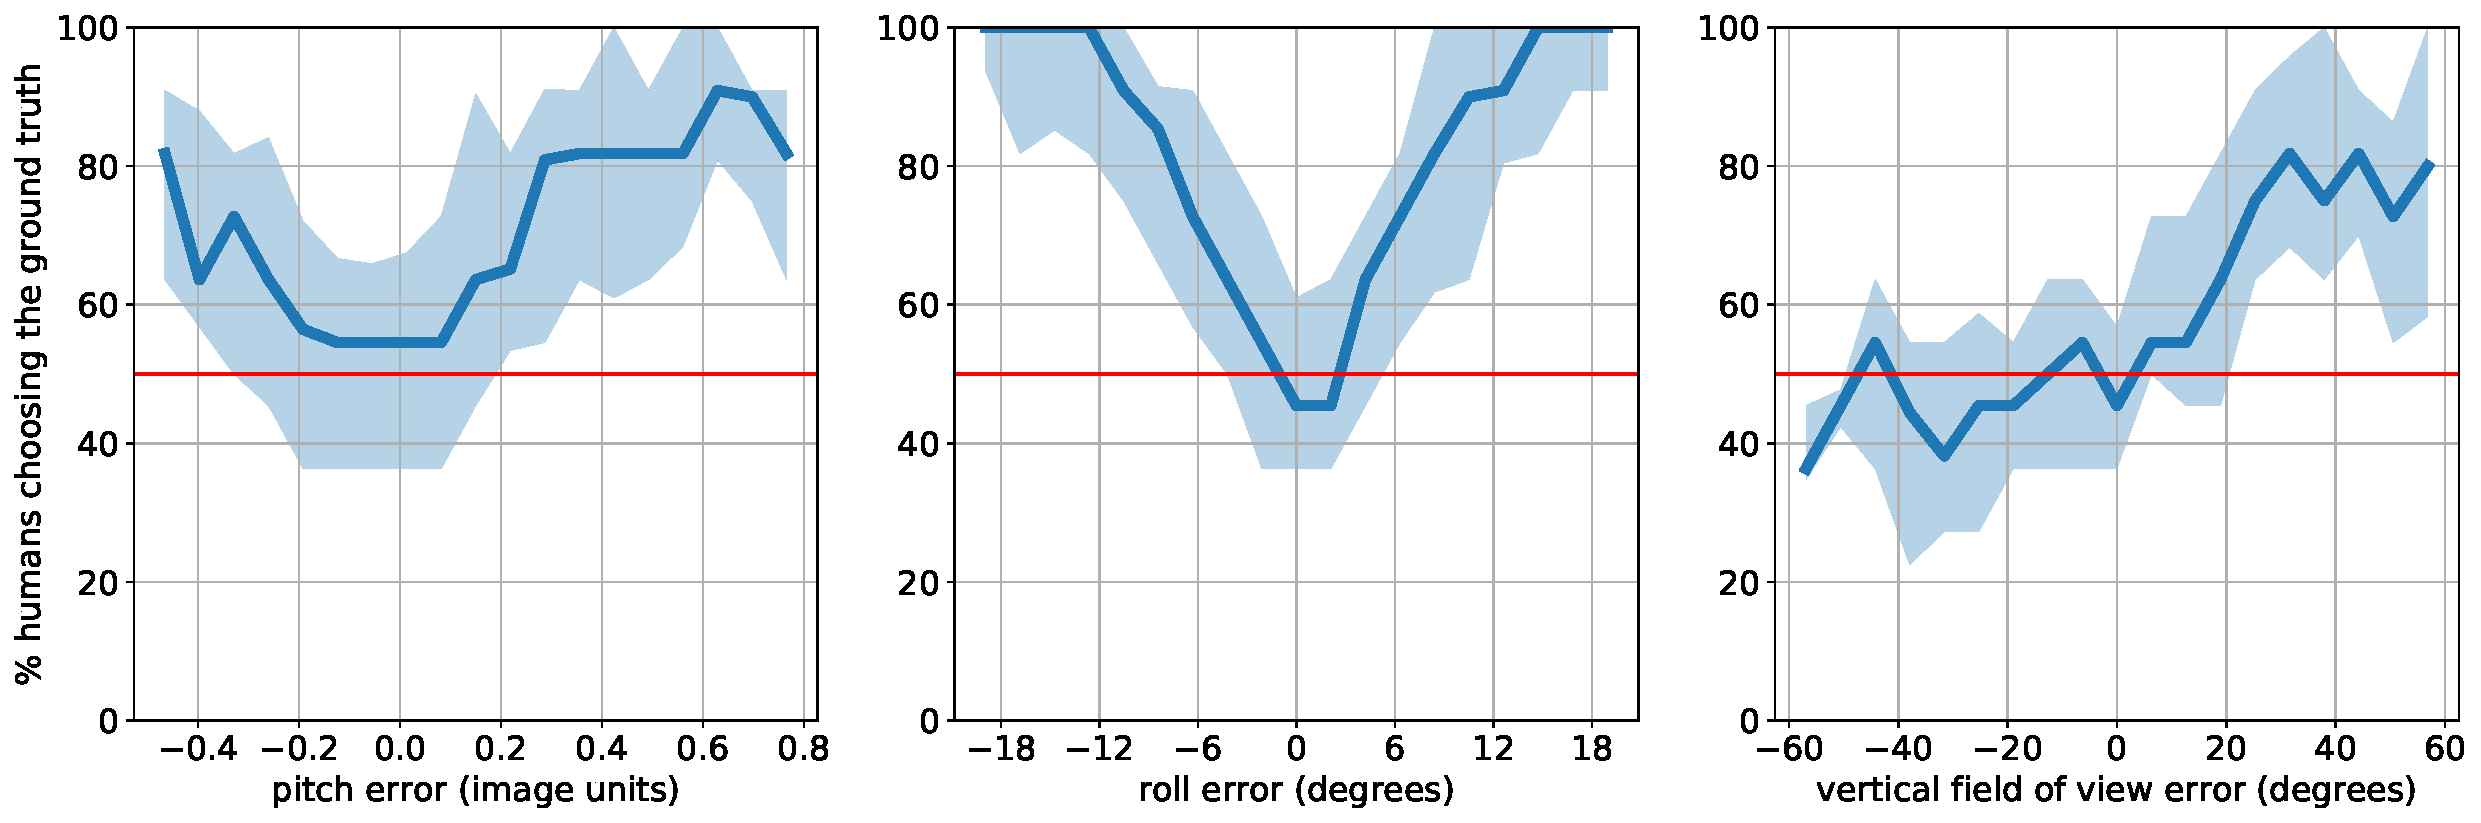
\includegraphics[width=\linewidth]{figures/pstudy/reduced_param_errors_pm_image_units_confusion.pdf} \\
\vspace{-0.1cm}
\begin{tabular}{p{0.3\linewidth}p{0.3\linewidth}p{0.3\linewidth}}
\hspace{1.15cm}(a) & \hspace{1cm}(b) & \hspace{0.85cm}(c)
\end{tabular}
\caption[Human sensitivity to calibration errors]{Human sensitivity to errors in (a) pitch, (b) roll and (c) field of view. We use the percentage of users choosing the image with an object inserted with the ground truth calibration as a measure of human sensitivity. 50\% represents confusion, meaning users are as likely to choose an insertion with a distorted calibration than the ground truth, and 100\% means that all humans could detect the ground truth image. The line represents the median of the percentage of people who pick the ground truth human for each image. The light shaded regions shows the first and third quartile.}
\label{fig:pstudy_overall_sensitivity}
\end{figure}


\paragraph{Error in camera parameters} We evaluate the sensitivity of humans to errors in camera parameters as a function of the errors in each parameter independently and illustrate the results in fig.~\ref{fig:pstudy_overall_sensitivity}. To generate this curve, we compute the percentage of times the study participants preferred the ground truth over the distorted image, and compute the median and percentiles across all images (and different virtual objects) that share the same amount of distortion. The higher the percentage in the $y$ axis, the more humans are prone to detect errors in this scenario. Conversely, 50\% indicates perfect confusion: participants are unable to distinguish between the ground truth and the distorted version. 

First, we note that when the error in camera parameters is close to 0, confusion nears 50\%, which is expected. What is interesting is how quickly sensitivity rises when increasing the error. We note a large tolerance to negative errors in field of view (fig.~\ref{fig:pstudy_overall_sensitivity}-c). Large positive errors (right side of the plot) translate in rendering an object with a field of view that is larger than that of the background. This results in increased perspective effects on the object, which tend to be visible. On the other hand, negative errors indicate that the perspective effect is \emph{not} as pronounced on the object as it should be with respect to the background image. In this scenario, participants seemed to have been unable to differentiate between the ground truth and the distorted object. For field of view, a range of $15\degree$ over and up to $50\degree$ under the ground truth value went unnoticed to the users.

Participants could tolerate an error in pitch up to 0.2 in rescaled image units (see sec.~\ref{sec:camera-model}), but beyond this threshold, users started to distinguish the distortions (fig.~\ref{fig:pstudy_overall_sensitivity}-a). The high sensitivity to roll errors is most prominent (fig.~\ref{fig:pstudy_overall_sensitivity}-b), where errors of $12\degree$ and more are almost systematically detected and only a small range of approximately $\pm2.5\degree$ roll error go unnoticed.


\begin{figure*}
\centering
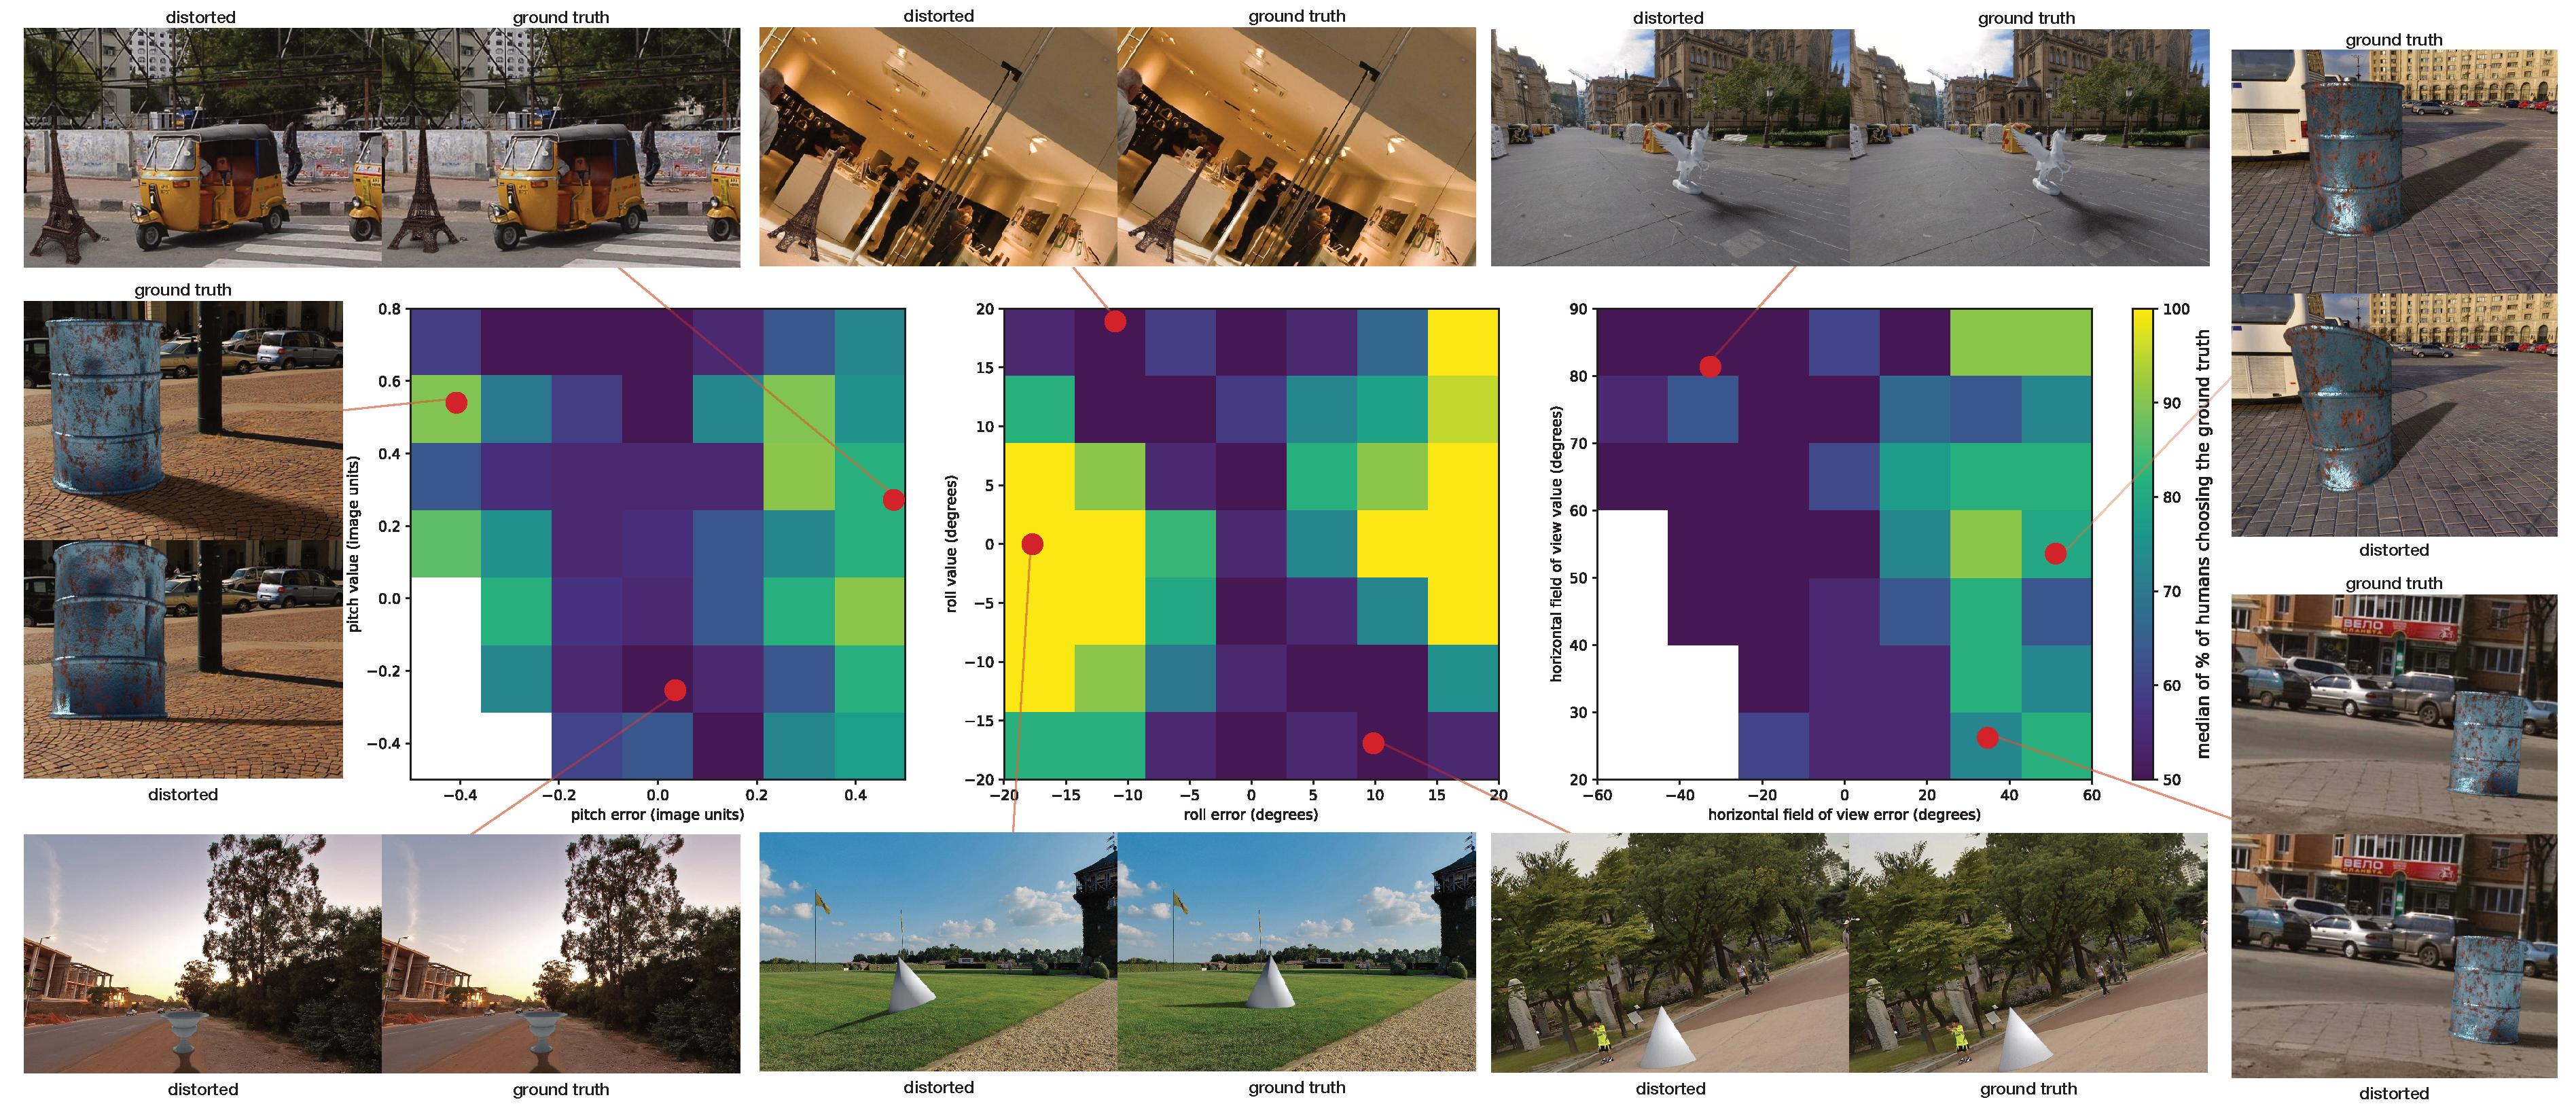
\includegraphics[width=\linewidth]{figures/pstudy/pstudy.pdf}
\caption[Human sensitivity to errors in calibration per parameter]{Human sensitivity to errors in pitch (left), roll (center) and field of view (right) as a function of individual parameter values, along with examples of image pairs shown to the users. We bin the percentage of people choosing the ground truth per image of the user study. The colors in the plot represents the median over all values in each bin. Note the strong relation between the roll value and its human sensitivity to error. Some combinations of parameters and errors makes it impossible to perform insertion leading to missing values in the figure (e.g., the ground is not visible anymore in the image (bottom left in pitch) or the resulting field of view would be too low or negative (bottom left in field of view)). \textbf{More examples available in annex~\ref{annex5}.}}
\label{fig:pstudy_sensitivity_per_parameter}
\end{figure*}

\paragraph{Joint space of error in camera parameters and absolute parameter value}

Evaluating sensitivity to errors in each parameter is interesting, but does not tell the whole story. Are there regions in parameter space where errors are more noticeable? To evaluate this, we plot the 2D space of errors and absolute parameter value in fig.~\ref{fig:pstudy_sensitivity_per_parameter}. The white squares in these plots are due to the fact that in these parameters configurations, the ground plane is not visible in the image and thus no virtual object can be inserted, so no perceptual data could be obtained.

First, our results suggest that human sensitivity to pitch error does not correlate strongly with horizon position in the image. Similarly, sensitivity to errors in field of view seems to be constant across all fields of view used in the study. However, the camera roll appears to have an influence on our perception of roll error. Indeed, images with high roll (in either direction) allow more room for roll estimation errors. 

\paragraph{}Please see the supplementary material for additional analysis, including joint modeling of distortions on multiple parameters.


\newcommand{\retrievalwidth}{0.12}
\begin{figure*}[!ht]
\centering
\footnotesize
\setlength{\tabcolsep}{3pt}
\begin{tabular}{c|cccc}
% \includegraphics[height=\retrievalwidth\linewidth]{figures/applications/matching_horizon_group_1/00003711_jpg_original.jpg} &
% \includegraphics[height=\retrievalwidth\linewidth]{figures/applications/matching_horizon_group_1/00000566_jpg_0_00466209680452972.jpg} &
% \includegraphics[height=\retrievalwidth\linewidth]{figures/applications/matching_horizon_group_1/00006763_jpg_0_0041125472055966875.jpg} &
% \includegraphics[height=\retrievalwidth\linewidth]{figures/applications/matching_horizon_group_1/00009395_jpg_0_004799502219410309.jpg} &
% \includegraphics[height=\retrievalwidth\linewidth]{figures/applications/matching_horizon_group_1/00023333_jpg_0_004026352908260552.jpg} \\
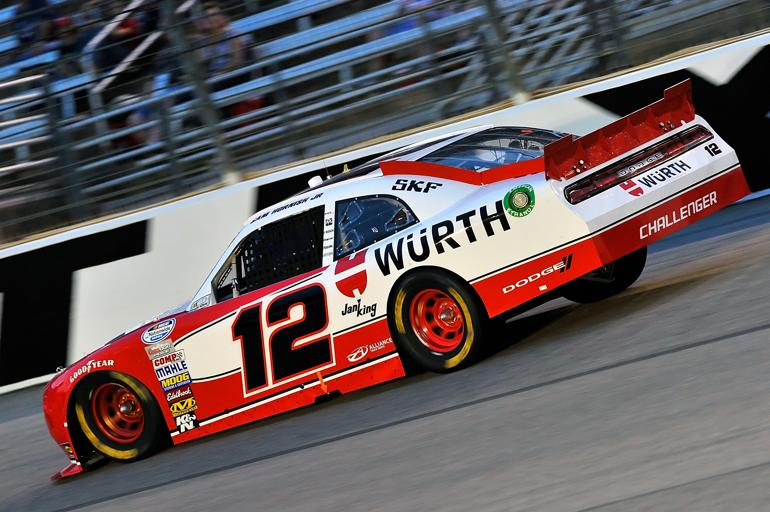
\includegraphics[height=\retrievalwidth\linewidth]{figures/applications/matching_horizon_group_3/00021396_jpg_0_46409649747812576_original.jpg} &
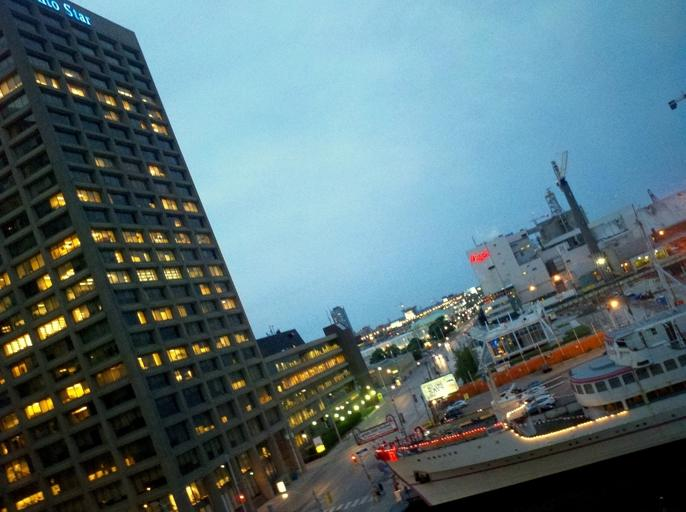
\includegraphics[height=\retrievalwidth\linewidth]{figures/applications/matching_horizon_group_3/00016279_jpg_0_07618561060718712.jpg} &
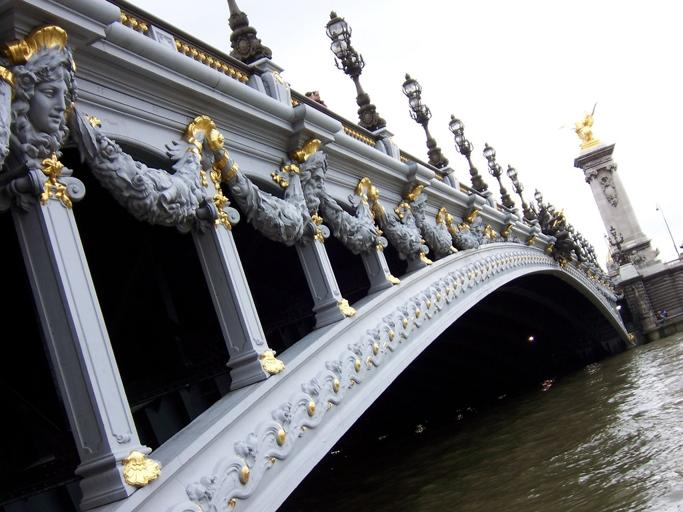
\includegraphics[height=\retrievalwidth\linewidth]{figures/applications/matching_horizon_group_3/00006311_jpg_0_06015428226537748.jpg} &
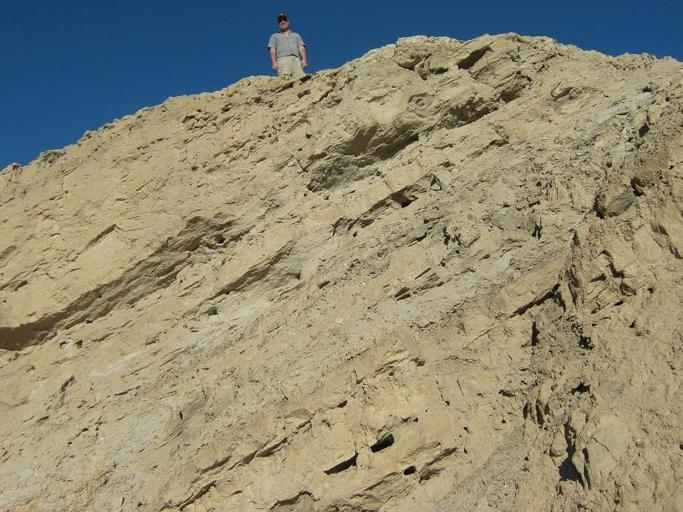
\includegraphics[height=\retrievalwidth\linewidth]{figures/applications/matching_horizon_group_3/00004613_jpg_0_10938281689401162.jpg} &
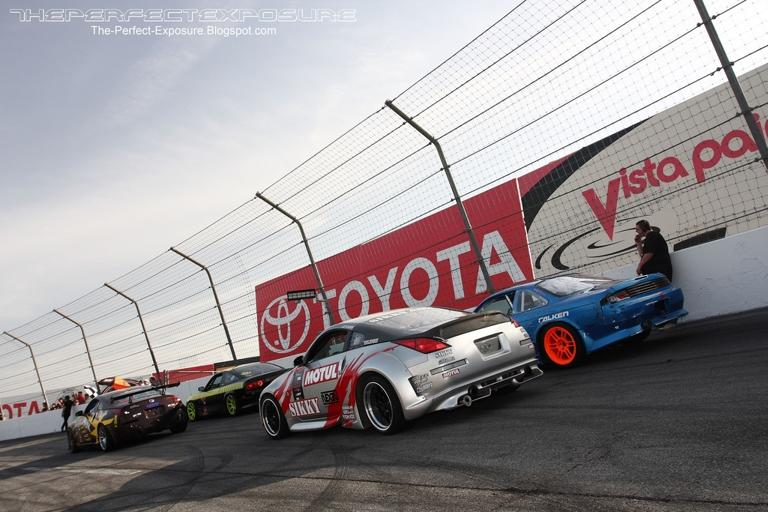
\includegraphics[height=\retrievalwidth\linewidth]{figures/applications/matching_horizon_group_3/00003549_jpg_0_040089855903650634.jpg} \\
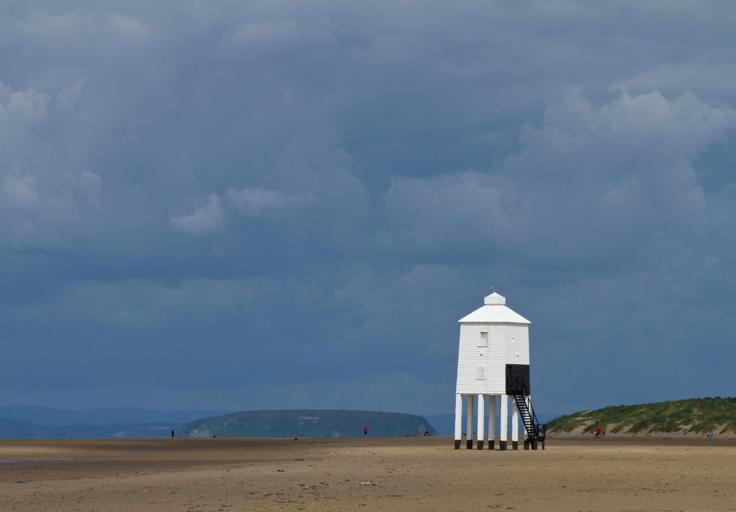
\includegraphics[height=\retrievalwidth\linewidth]{figures/applications/matching_horizon_group_2/00025416_jpg_original.jpg} &
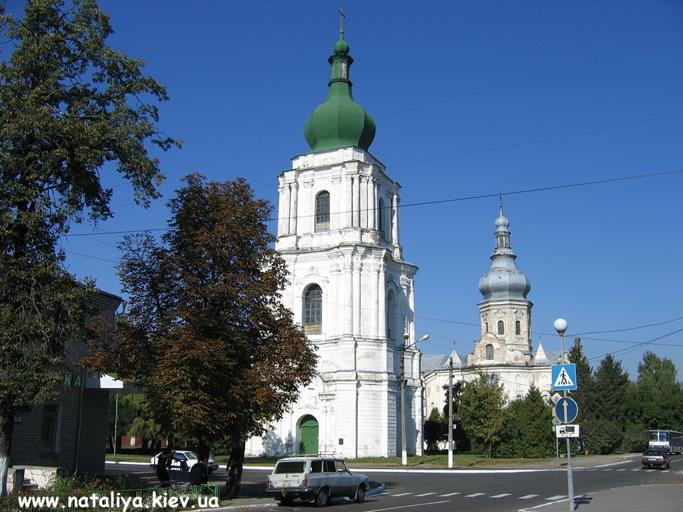
\includegraphics[height=\retrievalwidth\linewidth]{figures/applications/matching_horizon_group_2/00014759_jpg_0_0016924598703210684.jpg} &
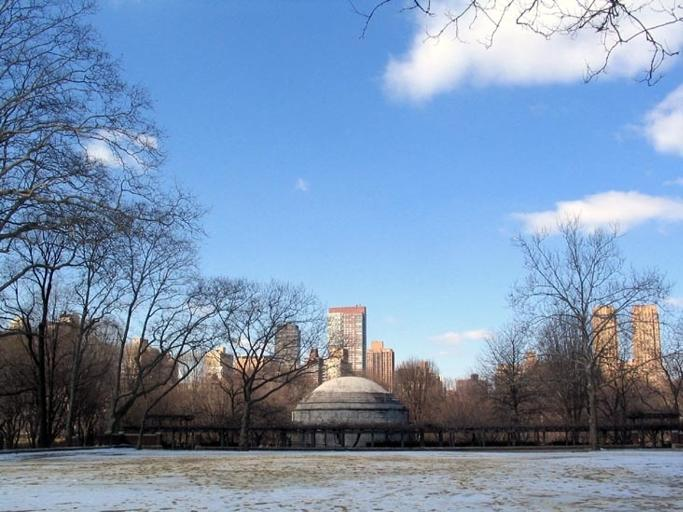
\includegraphics[height=\retrievalwidth\linewidth]{figures/applications/matching_horizon_group_2/00025187_jpg_0_002802485425429538.jpg} &
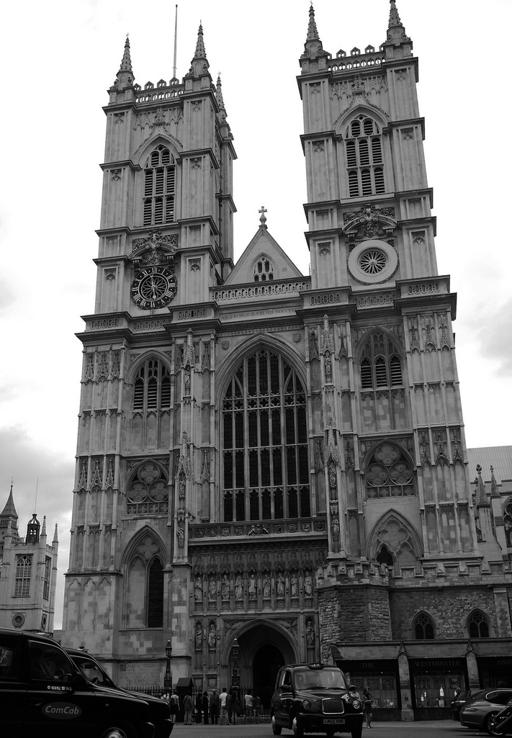
\includegraphics[height=\retrievalwidth\linewidth]{figures/applications/matching_horizon_group_2/00019725_jpg_0_0037706014462054725.jpg} &
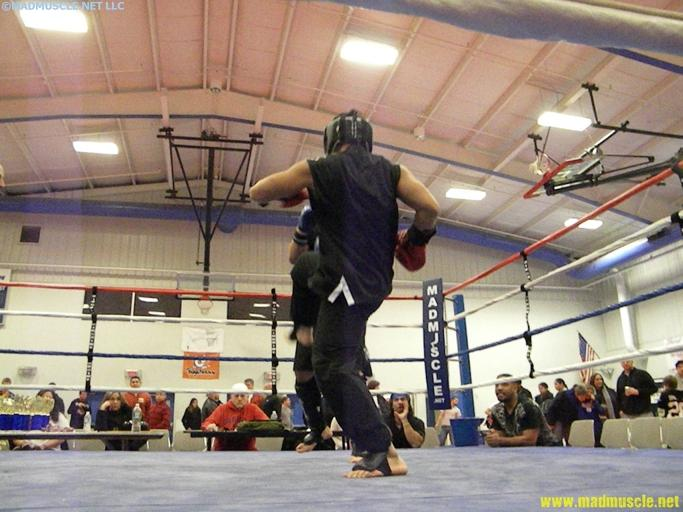
\includegraphics[height=\retrievalwidth\linewidth]{figures/applications/matching_horizon_group_2/00005226_jpg_0_004158961011695579.jpg} \\
Query & NN1 & NN2 & NN3 & NN4
\end{tabular}
\vspace{1em}
\caption[Examples of image retrieval]{Examples of image retrieval by horizon location on Places2. The horizon line is estimated using our method from the query image, and used to find closest matches in a 10k random subset from Places2. The top-4 matches are shown on the right.}
\label{fig:applications_retrieval}
\end{figure*}

